%% Source of figures/smote-decision-points.pdf. Compile: pdflatex smote-decision-points.tex
%% Figure 1 of the Method part draft (Claude, 29 Oct 2026): where each of the six decision
%% points acts on the SMOTE generation rule. (a) the rule, with each decision point pointing
%% at the symbol it changes; (b) the same six points on a two-dimensional sketch.
%% Numbers in circles keep the figure readable in black and white.
\documentclass[tikz,border=4pt]{standalone}
\usepackage[scaled]{helvet}\renewcommand{\familydefault}{\sfdefault}
\usepackage{amsmath,amssymb}
\usetikzlibrary{arrows.meta,positioning,fit,calc,shapes.geometric,backgrounds}
\definecolor{cSeed}{HTML}{2A78D6}\definecolor{cAlloc}{HTML}{EB6834}\definecolor{cNbr}{HTML}{1BAF7A}
\definecolor{cPlace}{HTML}{C98A00}\definecolor{cFilt}{HTML}{C0392B}\definecolor{cPipe}{HTML}{7B4FA0}
\definecolor{ink}{HTML}{17212B}\definecolor{inkTwo}{HTML}{465462}\definecolor{maj}{HTML}{A3ABB4}
\newcommand{\nb}[2]{\tikz[baseline=(n.base)]\node[circle,fill=#1,text=white,inner sep=0.6pt,minimum size=11pt,font=\scriptsize\bfseries](n){#2};}
\begin{document}
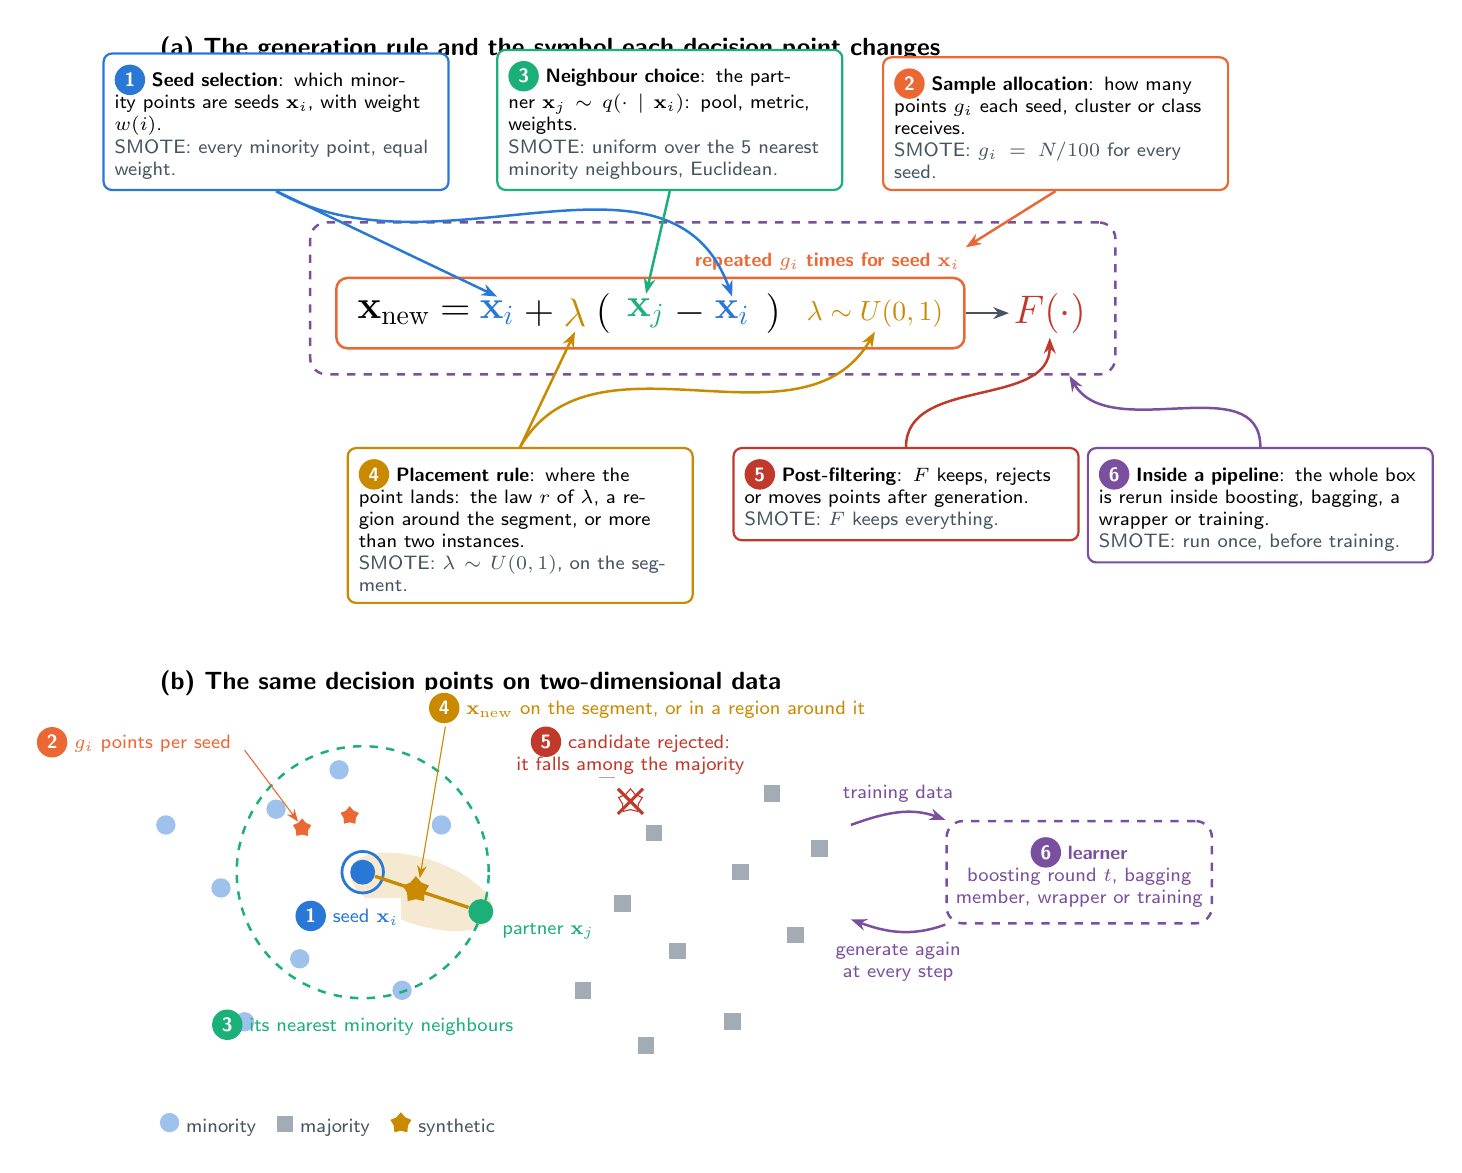
\begin{tikzpicture}[
  term/.style={inner sep=1.5pt,font=\Large},
  lbl/.style={draw=#1,rounded corners=3pt,fill=white,align=left,font=\scriptsize,text width=4.1cm,inner sep=4pt,line width=0.8pt},
  arr/.style={-{Stealth[length=2mm]},draw=#1,line width=0.9pt},
  ]
%% ---------------- panel (a): the rule ----------------
\node[font=\small\bfseries,anchor=west] at (-6.2,3.35) {(a) The generation rule and the symbol each decision point changes};
\node[term] (new) at (-3.1,0) {$\mathbf{x}_{\mathrm{new}}$};
\node[term,right=0pt of new] (eq) {$=$};
\node[term,right=0pt of eq,text=cSeed] (xi) {$\mathbf{x}_i$};
\node[term,right=0pt of xi] (plus) {$+$};
\node[term,right=0pt of plus,text=cPlace] (lam) {$\lambda$};
\node[term,right=0pt of lam] (lp) {$(\,$};
\node[term,right=0pt of lp,text=cNbr] (xj) {$\mathbf{x}_j$};
\node[term,right=0pt of xj] (mi) {$-$};
\node[term,right=0pt of mi,text=cSeed] (xi2) {$\mathbf{x}_i$};
\node[term,right=0pt of xi2] (rp) {$\,)$};
\node[term,right=6pt of rp,font=\normalsize,text=cPlace] (law) {$\lambda\sim U(0,1)$};
\node[draw=cAlloc,line width=0.9pt,rounded corners=4pt,fit=(new)(law),inner sep=6pt] (body) {};
\node[anchor=south east,font=\scriptsize\bfseries,text=cAlloc,inner sep=2pt] (rep) at (body.north east) {repeated $g_i$ times for seed $\mathbf{x}_i$};
\node[term,right=0.55cm of body,font=\Large,text=cFilt] (F) {$F(\cdot)$};
\draw[arr=inkTwo] (body.east) -- (F.west);
\node[draw=cPipe,dashed,line width=0.9pt,rounded corners=6pt,fit=(body)(F)(rep),inner sep=9pt] (pipe) {};
%% labels above
\node[lbl=cSeed,anchor=south] (L1) at (-4.6,1.55) {\nb{cSeed}{1}\ \textbf{Seed selection}: which minority points are seeds $\mathbf{x}_i$, with weight $w(i)$.\\ \textcolor{inkTwo}{SMOTE: every minority point, equal weight.}};
\node[lbl=cNbr,anchor=south] (L3) at (0.4,1.55) {\nb{cNbr}{3}\ \textbf{Neighbour choice}: the partner $\mathbf{x}_j\sim q(\cdot\mid\mathbf{x}_i)$: pool, metric, weights.\\ \textcolor{inkTwo}{SMOTE: uniform over the 5 nearest minority neighbours, Euclidean.}};
\node[lbl=cAlloc,anchor=south] (L2) at (5.3,1.55) {\nb{cAlloc}{2}\ \textbf{Sample allocation}: how many points $g_i$ each seed, cluster or class receives.\\ \textcolor{inkTwo}{SMOTE: $g_i=N/100$ for every seed.}};
%% labels below
\node[lbl=cPlace,anchor=north] (L4) at (-1.5,-1.7) {\nb{cPlace}{4}\ \textbf{Placement rule}: where the point lands: the law $r$ of $\lambda$, a region around the segment, or more than two instances.\\ \textcolor{inkTwo}{SMOTE: $\lambda\sim U(0,1)$, on the segment.}};
\node[lbl=cFilt,anchor=north] (L5) at (3.4,-1.7) {\nb{cFilt}{5}\ \textbf{Post-filtering}: $F$ keeps, rejects or moves points after generation.\\ \textcolor{inkTwo}{SMOTE: $F$ keeps everything.}};
\node[lbl=cPipe,anchor=north] (L6) at (7.9,-1.7) {\nb{cPipe}{6}\ \textbf{Inside a pipeline}: the whole box is rerun inside boosting, bagging, a wrapper or training.\\ \textcolor{inkTwo}{SMOTE: run once, before training.}};
\draw[arr=cSeed] (L1.south) -- (xi.north);
\draw[arr=cSeed] (L1.south) to[out=-30,in=110] (xi2.north);
\draw[arr=cNbr] (L3.south) -- (xj.north);
\draw[arr=cAlloc] (L2.south) -- (rep.north east);
\draw[arr=cPlace] (L4.north) -- (lam.south);
\draw[arr=cPlace] (L4.north) to[out=60,in=-120] (law.south);
\draw[arr=cFilt] (L5.north) to[out=90,in=-90] (F.south);
\draw[arr=cPipe] (L6.north) to[out=90,in=-60] ($(pipe.south east)+(-0.6,0)$);
%% ---------------- panel (b): geometric view ----------------
\begin{scope}[shift={(-5.6,-7.7)}]
\node[font=\small\bfseries,anchor=west] at (-0.6,3.0) {(b) The same decision points on two-dimensional data};
% majority points
\foreach \p in {(5.2,1.9),(5.8,1.1),(6.4,2.2),(6.9,0.6),(5.4,0.2),(7.3,1.6),(6.1,-0.4),(7.6,-0.2),(4.9,-0.9),(6.8,-1.3),(7.9,0.9),(5.7,-1.6)}
  \node[rectangle,fill=maj,minimum size=6pt,inner sep=0pt] at \p {};
% minority points
\foreach \p in {(0.3,0.4),(1.0,1.4),(1.3,-0.5),(2.1,0.6),(0.6,-1.3),(2.6,-0.9),(1.8,1.9),(3.1,1.2),(3.6,0.1),(-0.4,1.2)}
  \node[circle,fill=cSeed!45,minimum size=7pt,inner sep=0pt] at \p {};
% seed
\node[circle,fill=cSeed,minimum size=9pt,inner sep=0pt] (s) at (2.1,0.6) {};
\node[circle,draw=cSeed,line width=1pt,minimum size=15pt,inner sep=0pt] at (s) {};
\node[anchor=north,font=\scriptsize,text=cSeed,fill=white,inner sep=1pt] at ($(s)+(-0.2,-0.32)$) {\nb{cSeed}{1} seed $\mathbf{x}_i$};
% neighbourhood
\draw[cNbr,dashed,line width=0.9pt] (s) circle (1.6);
\node[font=\scriptsize,text=cNbr,anchor=north] at ($(s)+(0,-1.62)$) {\nb{cNbr}{3} its nearest minority neighbours};
% partner
\node[circle,fill=cNbr,minimum size=9pt,inner sep=0pt] (p) at (3.6,0.1) {};
\node[font=\scriptsize,text=cNbr,anchor=west] at ($(p)+(0.15,-0.25)$) {partner $\mathbf{x}_j$};
% segment and placement
\begin{scope}[on background layer]
\fill[cPlace!18,rotate around={-18.4:($(s)!0.5!(p)$)}] ($(s)!0.5!(p)$) ellipse (0.95 and 0.42);
\end{scope}
\draw[cPlace,line width=1.2pt] (s) -- (p);
\node[star,star points=5,fill=cPlace,minimum size=10pt,inner sep=0pt] (n1) at ($(s)!0.45!(p)$) {};
\node[font=\scriptsize,text=cPlace,anchor=south west,fill=white,inner sep=1pt] (nl) at (2.9,2.45) {\nb{cPlace}{4} $\mathbf{x}_{\mathrm{new}}$ on the segment, or in a region around it};
\draw[cPlace,-{Stealth[length=1.6mm]}] (nl.south west) ++(0.25,0) -- ($(n1)+(0.05,0.15)$);
% allocation: more points from one seed
\node[star,star points=5,fill=cAlloc,minimum size=7pt,inner sep=0pt] at ($(s)!0.7!(1.0,1.4)$) {};
\node[star,star points=5,fill=cAlloc,minimum size=7pt,inner sep=0pt] at ($(s)!0.55!(1.8,1.9)$) {};
\node[font=\scriptsize,text=cAlloc,anchor=east] at (0.55,2.25) {\nb{cAlloc}{2} $g_i$ points per seed};
\draw[cAlloc,-{Stealth[length=1.6mm]}] (0.6,2.15) -- ($(s)!0.7!(1.0,1.4)+(-0.05,0.08)$);
% rejected candidate
\node[star,star points=5,draw=cFilt,fill=white,minimum size=9pt,inner sep=0pt] (bad) at (5.5,1.5) {};
\draw[cFilt,line width=1.1pt] ($(bad)+(-0.16,-0.16)$) -- ($(bad)+(0.16,0.16)$) ($(bad)+(-0.16,0.16)$) -- ($(bad)+(0.16,-0.16)$);
\node[font=\scriptsize,text=cFilt,anchor=south,fill=white,inner sep=1pt,align=center] at ($(bad)+(0,0.3)$) {\nb{cFilt}{5} candidate rejected:\\ it falls among the majority};
% legend
\node[anchor=west,font=\scriptsize,text=inkTwo] at (-0.6,-2.6) {\tikz\node[circle,fill=cSeed!45,minimum size=7pt,inner sep=0pt]{}; minority\quad \tikz\node[rectangle,fill=maj,minimum size=6pt,inner sep=0pt]{}; majority\quad \tikz\node[star,star points=5,fill=cPlace,minimum size=8pt,inner sep=0pt]{}; synthetic};
% pipeline loop
\node[draw=cPipe,dashed,rounded corners=6pt,line width=0.9pt,align=center,font=\scriptsize,text=cPipe,minimum width=3.1cm,minimum height=1.3cm] (learn) at (11.2,0.6) {\nb{cPipe}{6} \textbf{learner}\\ boosting round $t$, bagging\\ member, wrapper or training};
\draw[cPipe,-{Stealth[length=2mm]},line width=0.9pt] (8.3,1.2) to[out=20,in=160] node[above,font=\scriptsize] {training data} (learn.north west);
\draw[cPipe,-{Stealth[length=2mm]},line width=0.9pt] (learn.south west) to[out=200,in=-20] node[below,font=\scriptsize,align=center] {generate again\\ at every step} (8.3,0.0);
\end{scope}
\end{tikzpicture}
\end{document}
